\begin{figure}[t]
\centering
\small
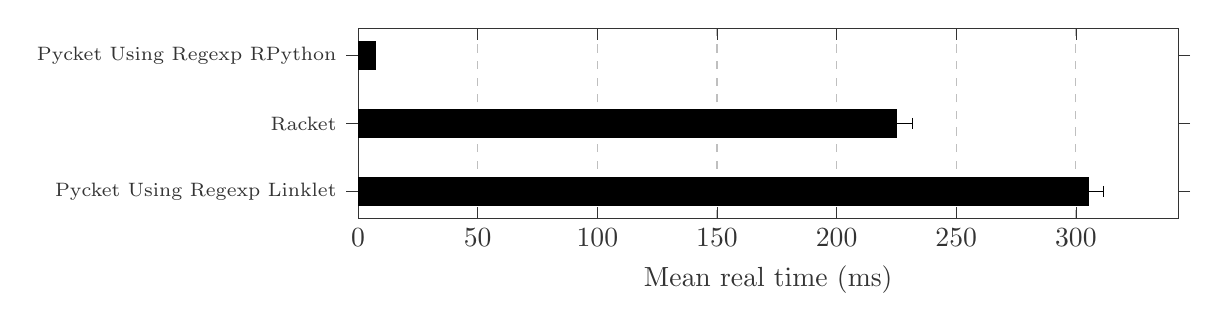
\begin{tikzpicture}
    \begin{axis}[
    xbar,
    xmin=0,
    width=12cm,
    height=4cm,
    xlabel={Mean real time (ms)},
    symbolic y coords={Pycket Using Regexp Linklet,Racket,Pycket Using Regexp RPython},
    ytick=data,
    bar width=10pt,
    xmajorgrids,
    grid style=dashed,
    % nodes near coords,
    % nodes near coords align={horizontal},
    % every node near coord/.append style={font=\footnotesize},
    tick style={black!80},
    axis line style={black!80},
    xlabel style={black!80},
    yticklabel style={font=\scriptsize, black!80},
    xticklabel style={black!80},
    enlarge y limits=0.2,
    ]
    % error-bar options live *inside* the plot style:
    \addplot+[
        black,
        error bars/.cd,
        x dir=both,
        x explicit,
        error bar style={black},
    ] coordinates {
        (305.25,Pycket Using Regexp Linklet) +- (  6.43,0)
        (225.05,Racket)                +- (  6.69,0)
        (  7.15,Pycket Using Regexp RPython) +- (  0.21,0)
    };
    \end{axis}
\end{tikzpicture}
\caption{Comparison of matching $\mathtt{\#}$\racketcode{rx"defg"} against a large \racketcode{"aaa...defg...aaa"} string -- lower is better.}
\label{fig:regexp-overall-comparison}
\end{figure}